\chapter*{Background}

\section*{Air Quality Monitors}
\addcontentsline{toc}{section}{Air Quality Monitors}
Air quality monitors are used to collect sensor data from different sources in the air. \cite{GeneralAirQualityMonitor} Air quality monitors can specialize in one measuring unit in the air or have the functionality to measure several air quality factors, such as gas, particulate pollutants, CO2, VOCs, humidity or temperature. The air quality monitors are incorporated in users homes and therefore the apperance of the device will also be a considerable factor for choosing the right device. \cite{IAQMonitorCommunicationReview} 
\\


\subsection*{Privacy and Security in Air Quality Monitors}
\addcontentsline{toc}{section}{Privacy and Security in Air Quality Monitors}
General security 
Encryption etc

Considering the amount of information an air quality monitor can collect about an individual or a smart home, privacy leakage is a vulnerability. \cite{SecPrivSmartCity} 


\subsection*{Private Information Inference}
\addcontentsline{toc}{subsection}{Private Information Inference}


\subsection*{Passive network Eavesdropping}
\addcontentsline{toc}{subsection}{Passive network Eavesdropping}

\section*{Communication Protocols}
\addcontentsline{toc}{section}{Communication Protocols}
Air Quality Monitors exists with different functionality and therefore also communicate over different communication protocols. Wi-Fi is the most preferred protocol with Bluetooth and Zigbee following. \cite{saini2020indoor} As this thesis is delimited to air quality monitor devices that uses Wi-Fi, Bluetooth, Zigbee or wired communication trough Ethernet as communication protocols, the next subsections will elaborate on these protocols and specifications to be used further in this thesis through testing and analysis. 

\subsection*{IEEE 802.11 - Wi-Fi}
\addcontentsline{toc}{subsection}{IEEE 802.11 - Wi-Fi}
Wireless Fidelity (Wi-Fi) \cite{WiFiAlliance} is one of the worlds most used technology for communicating and is defined, developed and standarized by WiFi Alliance. \cite{WiFiAlliance} Wi-Fi is based on the standard IEEE 802.11 Wireless LAN set by IEEE Standard for Information Technology. \cite{WifiStandard} The transmission range for Wi-Fi is up to 100 meters and it uses 5-60GHz in the frequency band. \cite{IAQMonitorCommunicationReview}

Wi-Fi packets transmitted follows the MAC frame format and is defined in Figure \ref{MACFrameFormat}. \cite{WifiStandard} 
\begin{figure}
    \centering
    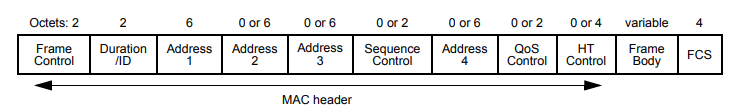
\includegraphics{figures/MACFrameFormat.png}
    \caption{MAC Frame Format \cite{WifiStandard}}
    \label{MACFrameFormat}
\end{figure}    

\subsection*{Bluetooth}
\addcontentsline{toc}{subsection}{Bluetooth}
The frequency band for Bluetooth is 2.4GHz and the transmission rate is up to 10 meters, which is relatively shorter compared to Wi-Fi. \cite{IAQMonitorCommunicationReview}

\subsection*{ZigBee}
\addcontentsline{toc}{subsection}{ZigBee}
ZigBee is also a popular choice for communication protocol when it comes to IoT devices. The protocol is based on the IEEE802.15.4 standard set by IEEE Standard for Information Technology. \cite{ZigBeeStandard} ZigBee uses the same frequency band as Bluetooth, 2.4GHz, but does obtain a longer transmission rate up to 20 meters. \cite{IAQMonitorCommunicationReview} 

\subsection*{Ethernet}
\addcontentsline{toc}{subsection}{Ethernet}

\subsection*{Comparison of the different communication protocols}
\addcontentsline{toc}{subsection}{Comparison of the different communication protocols}
In Table \ref{CommunicationProtocolsComparison} a comparison of the different communication protocols that will be used during tests in this thesis and their specifications are presented. \\
\begin{table}[!hbtp]
\begin{tabular}{||c | c | c ||} 
 \hline
 Communication Protocol & Frequency Band & Transmission Range  \\ [0.5ex]
 \hline\hline
 Wi-Fi & 5-60GHz & 100m \\ 
 Bluetooth & 2.4GHz & 10m \\
 ZigBee & 2.4GHz & 20m \\
 Ethernet & ? & NA \\ [1ex] 
 \hline
\end{tabular}
\caption{Communication Protocols Comparison}
\label{CommunicationProtocolsComparison}
\end{table}